\documentclass[letterpaper,11pt]{article}
\usepackage{geometry}   % See geometry.pdf to learn the layout
                        % options.  There are lots.
\usepackage[latin1]{inputenc}
\usepackage{graphicx}
\usepackage{epstopdf}
\usepackage{amsmath,amsfonts,amssymb}

\DeclareGraphicsRule{.tif}{png}{.png}{`convert #1 `dirname #1`/`basename #1 .tif`.png}

\author{Daniel R. Reynolds}
\title{Flux Limter Formulations and Results}

\textheight 9truein
\textwidth 6.5truein
\addtolength{\oddsidemargin}{-0.25in}
\addtolength{\evensidemargin}{-0.25in}
\addtolength{\topmargin}{-0.5in}
\setlength{\parindent}{0em}
\setlength{\parskip}{2ex}


\begin{document}
\maketitle

\section{Limiter Formulation}
\label{sec:model}

We consider a model of flux-limited diffusion for radiation transport
in a cosmological medium,
\begin{equation}
\label{eq:FLD_eqn}
  \partial_t E = \nabla\cdot\left(D\nabla E\right) - \frac{\dot{a}}{a}E - c \kappa E + \eta,
\end{equation}
where here $E$ is the comoving grey radiation energy density.  Within
this equation, the function $D$ is the {\em flux limiter} that depends on $E$,
$\nabla E$ and the opacity $\kappa$.  We compute this
limiter at each face of every finite-volume cell, where for a face
adjoining two cells containing the radiation values $E_1$ and $E_2$,
and the opacity values $\kappa_1$ and $\kappa_2$,
\begin{align}
  D &= \min\left\{ c \left(9\kappa^2 + R^2\right)^{-1/2} , D_{max} \right\}, \\
  R &= \max\left\{\frac{|E_2-E_1|}{\Delta x E}, R_{min}\right\}, \\
  E &= \max\left\{ \frac{E_1+E_2}{2}, E_{min} \right\}, \\
  \kappa &= \frac{2 \kappa_1 \kappa_2}{\kappa_1 + \kappa_2}.
\end{align}
In the above formulas, we have the fixed parameter values $E_{min}$
(dimensionless), $R_{min}$ (dimensions of cm$^{-1}$) and $D_{max}$
(dimensions of cm$^2$ s$^{-1}$).




\section{Variations on the Limiter Bounds}
\label{sec:bounds}

We have been investigating alternate formulations for the limiter
bound constants $R_{min}$, $E_{min}$ and $D_{max}$.  In our original
formulation of the solver, these constants had the following values:
\begin{itemize}
\item $R_{min} = 10^{-20}$
\item $E_{min} = 0$
\item $D_{max} = \infty$
\end{itemize}
These values passed all of our initial tests, and seemed to provide
highly reliable results.  A primary concern, however, was the use of
the fixed constant $R_{min} = 10^{-20}$, regardless of the length
units in the problem, even though $R_{min}$ itself should have units
of cm$^{-1}$.

Unfortunately, when attempting the two new test problems of an
expanding HII region in a cosmological density field, and the
photoevaporation of a dense HI clump, our solver produced entirely
non-physical results.  These plots will be included in the comparisons
in section \ref{sec:results}.  

We have therefore investigated a wide variety of alternate
formulations of these limiter bounds.  Of our myriad tests, we have
converged to three different possible formulations of these limiter
bounds.  In each of these formulations, we make use of Enzo's
problem-dependent non-dimensionalization constants,
\begin{itemize}
\item $L_{unit}$ -- length unit nondimensionalization factor
\item $T_{unit}$ -- time unit nondimensionalization factor
\end{itemize}
along with the speed of light, $c=2.99792458\cdot 10^{10}$ cm
s$^{-1}$. 



\subsection{Variation 1}
\label{sec:var1}

Our first reformulation of the limiter bounds adds in the unused bounds
from before, and creates bounds with the correct units,
\begin{itemize}
\item $R_{min} = 10^{-20} / L_{unit}$,
\item $E_{min} = 10^{-30}$,
\item $D_{max} = \alpha\, c\, L_{unit}$,
\end{itemize}
where $\alpha$ is a yet-to-be-specified nondimensional constant.


\subsection{Variation 2}
\label{sec:var2}

Our second reformulation of the limiter bounds is a modification of the
previous one, that uses a different approach for creating the
dimensional boud $D_{max}$,
\begin{itemize}
\item $R_{min} = 10^{-20} / L_{unit}$,
\item $E_{min} = 10^{-30}$,
\item $D_{max} = \beta\, L_{unit}^2 / T_{unit}$,
\end{itemize}
where $\beta$ is a yet-to-be-specified nondimensional constant.


\subsection{Variation 3}
\label{sec:var3}

Our final reformulation of the limiter bounds is a hybrid of the
preceding two approaches,
\begin{itemize}
\item $R_{min} = 10^{-20} / L_{unit}$,
\item $E_{min} = 10^{-30}$,
\item $D_{max} = \gamma\, c\, L_{unit} + \delta\, L_{unit}^2 / T_{unit}$,
\end{itemize}
where again $\gamma$ and $\delta$ are yet-to-be-specified
nondimensional constants. 



\section{Results}
\label{sec:results}


In the following subsections, we compare results from the above four
formulations of the flux limiter bounds (original and variations 1-3),
along with corresponding results from Enzo's ray-tracing solver on the
same problems.  For both of the limiter bound variations 1 and 2, we
will show two different sets of $\alpha$ and $\beta$ values, each
tuned to one of the test problems of interest (but that perform poorly
on the other test problem).  As a result, we will compare 7 total
results on each metric:
\begin{itemize}
\item[(0)] Ray-Tracing solver,
\item[(A)] Variation 1, with $\alpha = 0.0060530$,
\item[(B)] Variation 1, with $\alpha = 0.0021620$,
\item[(C)] Variation 2, with $\beta = 0.025979$,
\item[(D)] Variation 2, with $\beta = 6.6287$,
\item[(E)] Variation 3, with $\gamma = 0.0021565$ and $\delta = 0.0167231$.
\item[(F)] Original formulation,
\end{itemize}



\subsection{Test 4 -- Multiple sources in a cosmological density field}
\label{sec:test4}

This is a HII ionization test in a static cosmological density
field.  The dimensionless contants for approaches A, C and E have been
tuned for this problem, but approaches B and D do not provide
as high quality of results.

We note that this test has unit non-dimensionalization factors:
\begin{itemize}
\item $L_{unit} = 2.20429\times10^{23}$
\item $T_{unit} = 3.1557\times10^{13}$
\end{itemize}
With these factors, we will have the following values of the limiter
bound $D_{max}$:
\begin{itemize}
\item[(A)] $D_{max} = 4\times10^{31}$
\item[(B)] $D_{max} = 1.4287\times10^{31}$
\item[(C)] $D_{max} = 4\times10^{31}$
\item[(D)] $D_{max} = 1.0206\times10^{34}$
\item[(E)] $D_{max} = 4\times10^{31}$
\item[(F)] $D_{max} = \infty$
\end{itemize}


\begin{figure}[t]
  \centerline{
  \includegraphics[scale=1.5, trim=0.0cm 0.0cm 0.0cm 0.0cm]{test4_IFracHist.png}
  }
  \caption{(Test 4) Ionized fraction history from the ray-tracing
    solver.  Results show both mass-averaged (dashed) and
    volume-averaged (solid) values.}
  \label{fig:test4_IFrac_RT}
\end{figure}

\begin{figure}[t]
  \centerline{\hfill
  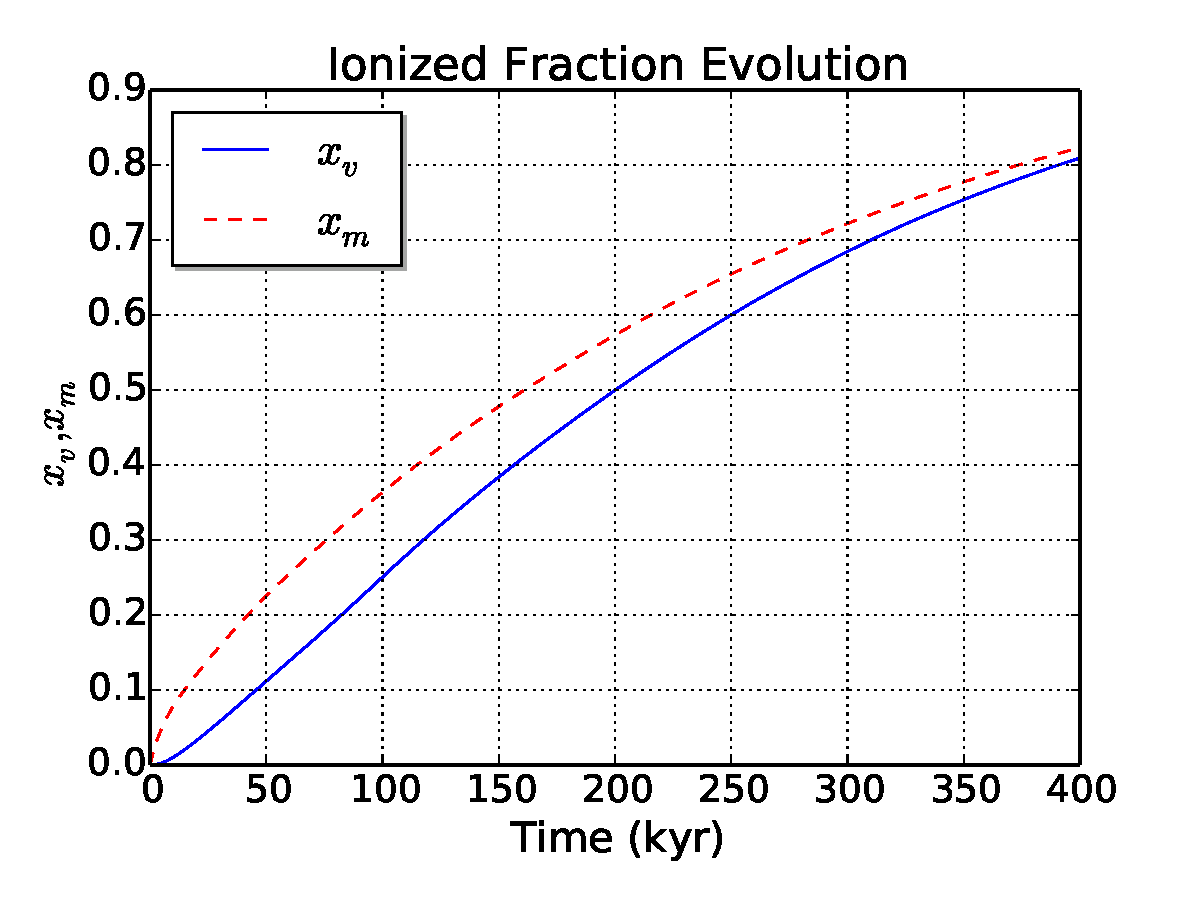
\includegraphics[scale=0.5, trim=0.0cm 0.0cm 0.0cm 0.0cm]{test4_IFracHist_A.png}
  \includegraphics[scale=0.5, trim=0.0cm 0.0cm 0.0cm 0.0cm]{test4_IFracHist_B.png}
  \hfill}
  \centerline{\hfill
  \includegraphics[scale=0.5, trim=0.0cm 0.0cm 0.0cm 0.0cm]{test4_IFracHist_C.png}
  \includegraphics[scale=0.5, trim=0.0cm 0.0cm 0.0cm 0.0cm]{test4_IFracHist_D.png}
  \hfill}
  \centerline{\hfill
  \includegraphics[scale=0.5, trim=0.0cm 0.0cm 0.0cm 0.0cm]{test4_IFracHist_E.png}
  \includegraphics[scale=0.5, trim=0.0cm 0.0cm 0.0cm 0.0cm]{test4_IFracHist_orig.png}
  \hfill}
  \caption{(Test 4) Ionized fraction history from the FLD approaches:
    first row are approaches A and B; second are C and D, third are E
    and F. Note that only A, C and E are close to the correct speed,
    while B and F are too slow, and D is too fast.} 
  \label{fig:test4_IFrac}
\end{figure}


\begin{figure}[t]
  \centerline{
  \includegraphics[scale=1.5, trim=1.0cm 0.0cm 0.0cm 0.0cm]{test4_PDF.png}
  }
  \caption{(Test 4) Probability density functions for neutral fraction
    and temperature at 50 kyr (solid line) and 200 kyr (dashed line)
    from the ray-tracing solver.} 
  \label{fig:test4_PDF_RT}
\end{figure}

\begin{figure}[t]
  \centerline{\hfill
  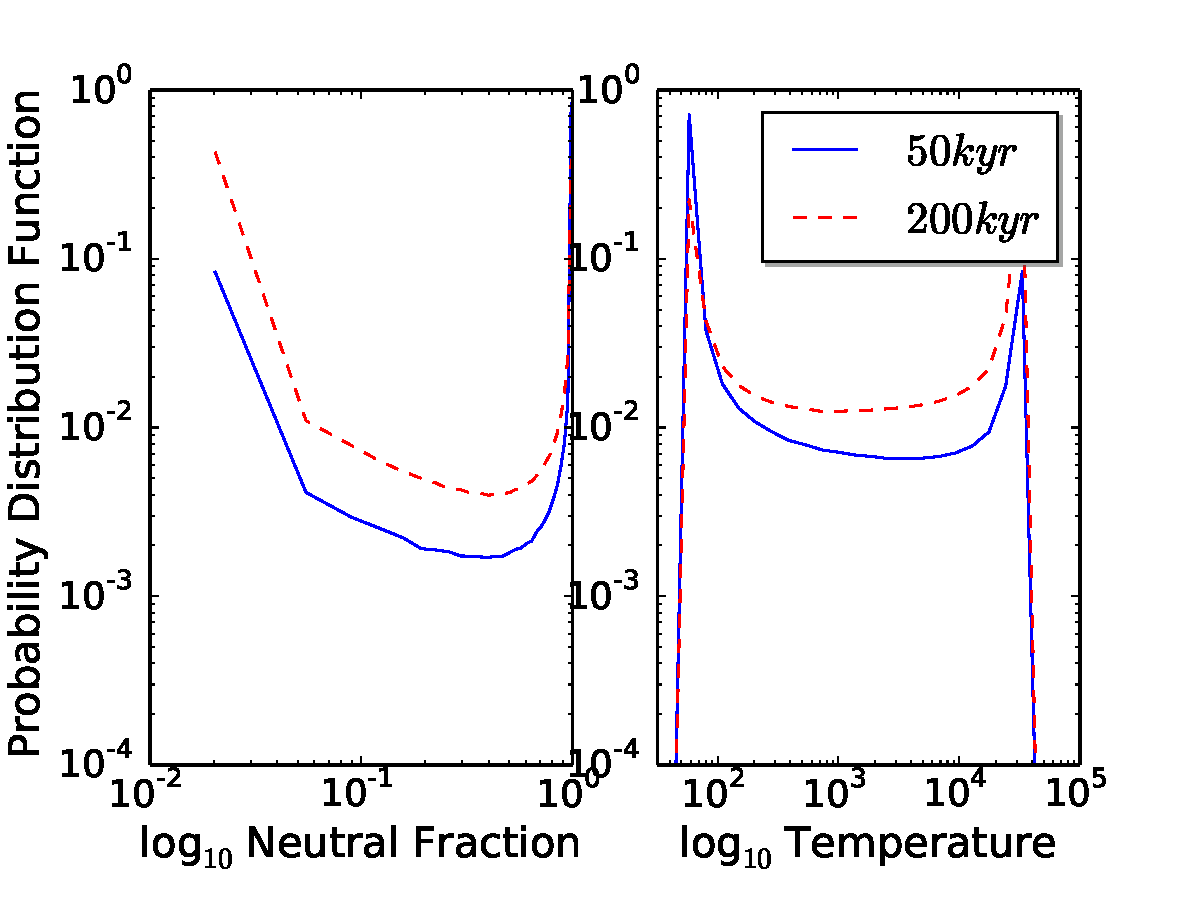
\includegraphics[scale=0.5, trim=0.0cm 0.0cm 0.0cm 0.0cm]{test4_PDF_A.png}
  \includegraphics[scale=0.5, trim=0.0cm 0.0cm 0.0cm 0.0cm]{test4_PDF_B.png}
  \hfill}
  \centerline{\hfill
  \includegraphics[scale=0.5, trim=0.0cm 0.0cm 0.0cm 0.0cm]{test4_PDF_C.png}
  \includegraphics[scale=0.5, trim=0.0cm 0.0cm 0.0cm 0.0cm]{test4_PDF_D.png}
  \hfill}
  \centerline{\hfill
  \includegraphics[scale=0.5, trim=0.0cm 0.0cm 0.0cm 0.0cm]{test4_PDF_E.png}
  \includegraphics[scale=0.5, trim=0.0cm 0.0cm 0.0cm 0.0cm]{test4_PDF_orig.png}
  \hfill}
  \caption{(Test 4) Probability density functions for neutral fraction
    and temperature from the FLD approaches: first row are approaches
    A and B; second are C and D, third are E and F.}
  \label{fig:test4_PDF}
\end{figure}


\begin{figure}[t]
  \centerline{
  \includegraphics[scale=1.0, trim=0.0cm 0.0cm 0.0cm 0.0cm]{test4_slices.png}
  }
  \caption{(Test 4) Slices through the origin of the neutral fraction
    and temperature at 50 and 200 kyr from the ray-tracing solver.}
  \label{fig:test4_slices_RT}
\end{figure}

\begin{figure}[t]
  \centerline{\hfill
  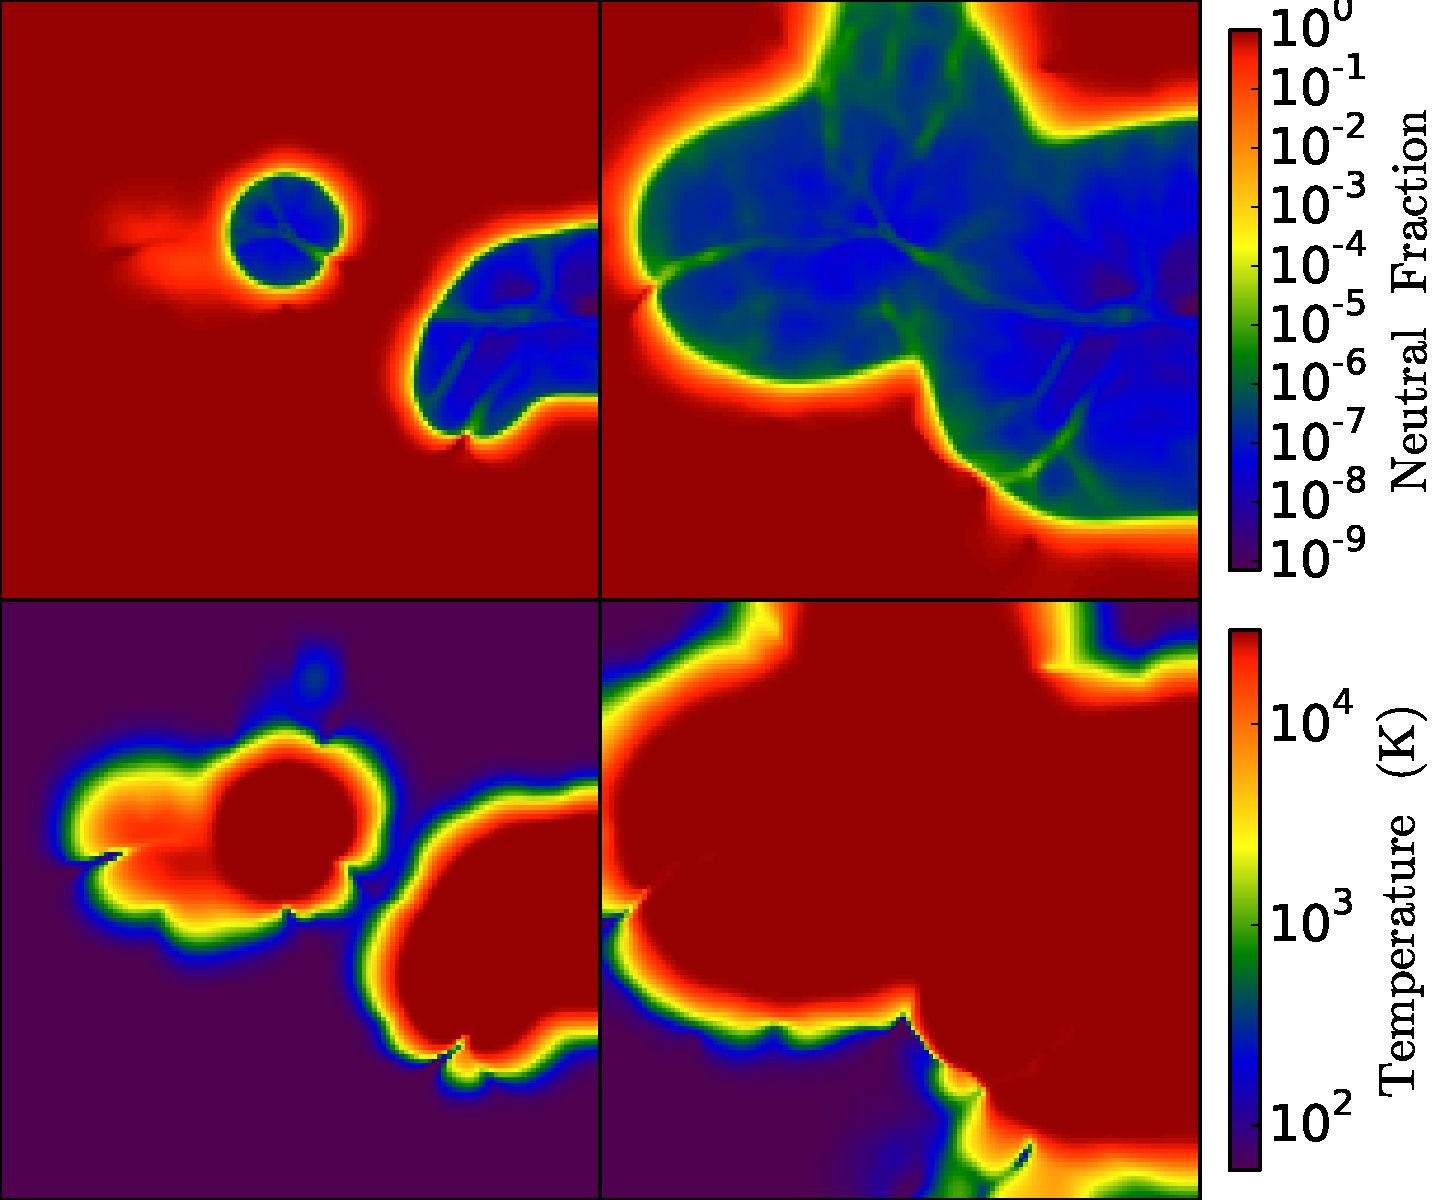
\includegraphics[scale=0.35, trim=0.0cm 0.0cm 0.0cm 0.0cm]{test4_slices_A.png}
  \includegraphics[scale=0.35, trim=0.0cm 0.0cm 0.0cm 0.0cm]{test4_slices_B.png}
  \hfill}
  \centerline{\hfill
  \includegraphics[scale=0.35, trim=0.0cm 0.0cm 0.0cm 0.0cm]{test4_slices_C.png}
  \includegraphics[scale=0.35, trim=0.0cm 0.0cm 0.0cm 0.0cm]{test4_slices_D.png}
  \hfill}
  \centerline{\hfill
  \includegraphics[scale=0.35, trim=0.0cm 0.0cm 0.0cm 0.0cm]{test4_slices_E.png}
  \includegraphics[scale=0.35, trim=0.0cm 0.0cm 0.0cm 0.0cm]{test4_slices_orig.png}
  \hfill}
  \caption{(Test 4) Slices through the origin of the neutral fraction
    and temperature at 50 and 200 kyr from the FLD approaches: first
    row are approaches A and B; second are C and D, third are E and
    F.  Note that again, A, C and E are closer to the ray-tracing
    results, B and F are too slow, and D is too fast (and exhibits a
    box-shaped front).}
  \label{fig:test4_slices}
\end{figure}




\subsection{Test 7 -- photoevaporation of a dense clump}
\label{sec:test7}

This is	a HII ionization test where the density field exhibits two
homogeneous regions: a high-density ``clump'' at approximately 2/3 of
the way to the right, and a surrounding low-density region.  At the
start of the simulation the field is fully neutral, and a point
source of radiation is placed at the left boundary of the domain.
This quickly ionizes the low density region, and eventually hits the
clump, which it ionizes more slowly.  

The dimensionless contants for approaches B, D and E have been
tuned for this problem, but approaches A and C do not provide
as high quality of results.

We note that this test has unit non-dimensionalization factors:
\begin{itemize}
\item $L_{unit} = 3.0857\times10^{21}$
\item $T_{unit} = 3.15576\times10^{14}$
\end{itemize}
With these factors, we will have the following values of the limiter
bound $D_{max}$:
\begin{itemize}
\item[(A)] $D_{max} = 5.5994\times10^{29}$
\item[(B)] $D_{max} = 2\times10^{29}$
\item[(C)] $D_{max} = 7.8384\times10^{26}$
\item[(D)] $D_{max} = 2\times10^{29}$
\item[(E)] $D_{max} = 2\times10^{29}$
\item[(F)] $D_{max} = \infty$
\end{itemize}


\begin{figure}[t]
  \centerline{
  \includegraphics[scale=1.0, trim=0.0cm 0.0cm 0.0cm 0.0cm]{test7_slices.png}
  }
  \caption{(Test 7) Slices through the dense clump of the neutral
    fraction, pressure, temperature and density at time 10 Myr from
    the ray-tracing solver.} 
  \label{fig:test7_slices_RT}
\end{figure}

\begin{figure}[t]
  \centerline{
  \includegraphics[scale=0.35, trim=0.0cm 0.0cm 0.0cm 0.0cm]{test7_slices_A.png}
  \includegraphics[scale=0.35, trim=0.0cm 0.0cm 0.0cm 0.0cm]{test7_slices_B.png}
  }
  \centerline{
  \includegraphics[scale=0.35, trim=0.0cm 0.0cm 0.0cm 0.0cm]{test7_slices_C.png}
  \includegraphics[scale=0.35, trim=0.0cm 0.0cm 0.0cm 0.0cm]{test7_slices_D.png}
  }
  \centerline{
  \includegraphics[scale=0.35, trim=0.0cm 0.0cm 0.0cm 0.0cm]{test7_slices_E.png}
  \includegraphics[scale=0.35, trim=0.0cm 0.0cm 0.0cm 0.0cm]{test7_slices_orig.png}
  }
  \caption{(Test 7) Slices through the dense clump of the neutral
    fraction, pressure, temperature and density at time 10 Myr from
    the FLD approaches: first row are approaches A and B; second are C
    and D, third are E and F. Note that now, B, D and E are closer to
    the ray-tracing results, while A and F are too fast, and C is too slow.} 
  \label{fig:test7_slices}
\end{figure}



\begin{figure}[t]
  \centerline{
  \includegraphics[scale=1.5, trim=0.0cm 0.0cm 0.0cm 0.0cm]{test7_profiles.png}
  }
  \caption{(Test 7) Profiles of the density, temperature, neutral
    fraction and pressure, as line cuts through the middle of the
    dense clump at different times from the ray-tracing solver.  The
    times 1, 10 and 50 Myr are plotted.} 
  \label{fig:test7_profiles_RT}
\end{figure}

\begin{figure}[t]
  \centerline{
  \includegraphics[scale=0.45, trim=0.0cm 0.0cm 0.0cm 0.0cm]{test7_profiles_A.png}
  \includegraphics[scale=0.45, trim=0.0cm 0.0cm 0.0cm 0.0cm]{test7_profiles_B.png}
  }
  \centerline{
  \includegraphics[scale=0.45, trim=0.0cm 0.0cm 0.0cm 0.0cm]{test7_profiles_C.png}
  \includegraphics[scale=0.45, trim=0.0cm 0.0cm 0.0cm 0.0cm]{test7_profiles_D.png}
  }
  \centerline{
  \includegraphics[scale=0.45, trim=0.0cm 0.0cm 0.0cm 0.0cm]{test7_profiles_E.png}
  \includegraphics[scale=0.45, trim=0.0cm 0.0cm 0.0cm 0.0cm]{test7_profiles_orig.png}
  }
  \caption{(Test 7) Profiles of the density, temperature, neutral
    fraction and pressure, as line cuts through the middle of the
    dense clump at different times from the FLD approaches: first row
    are approaches A and B; second are C and D, third are E and F.
    The times 1, 5 and 10 Myr are plotted; line styles have been
    chosen to match figure \ref{fig:test7_profiles_RT}.  Note that as
    in figure \ref{fig:test7_slices}, B, D and E are closer to
    the ray-tracing results, while A and F are too fast, and C is too slow.} 
  \label{fig:test7_profiles}
\end{figure}



\subsection{Consolidated HII test}
\label{sec:ConsolidatedTest}

This is also a HII ionization test, where the density field is
homogeneous, and two point sources are placed in the domain. The test
watches the merger of the two spherical ionized regions.  

All approaches for the limiter bounds seem to give the correct results
on this problem, though formulation E took too long to run and the job
was stopped. 

We note that this test has unit non-dimensionalization factors:
\begin{itemize}
\item $L_{unit} = 3.0857\times10^{22}$
\item $T_{unit} = 10^{16}$
\end{itemize}
With these factors, we will have the following values of the limiter
bound $D_{max}$:
\begin{itemize}
\item[(A)] $D_{max} = 5.5994\times10^{30}$
\item[(B)] $D_{max} = 2\times10^{30}$
\item[(C)] $D_{max} = 2.4736\times10^{27}$
\item[(D)] $D_{max} = 6.3115\times10^{29}$
\item[(E)] $D_{max} = 1.9965\times10^{30}$
\item[(F)] $D_{max} = \infty$
\end{itemize}


\begin{figure}[t]
  \centerline{
  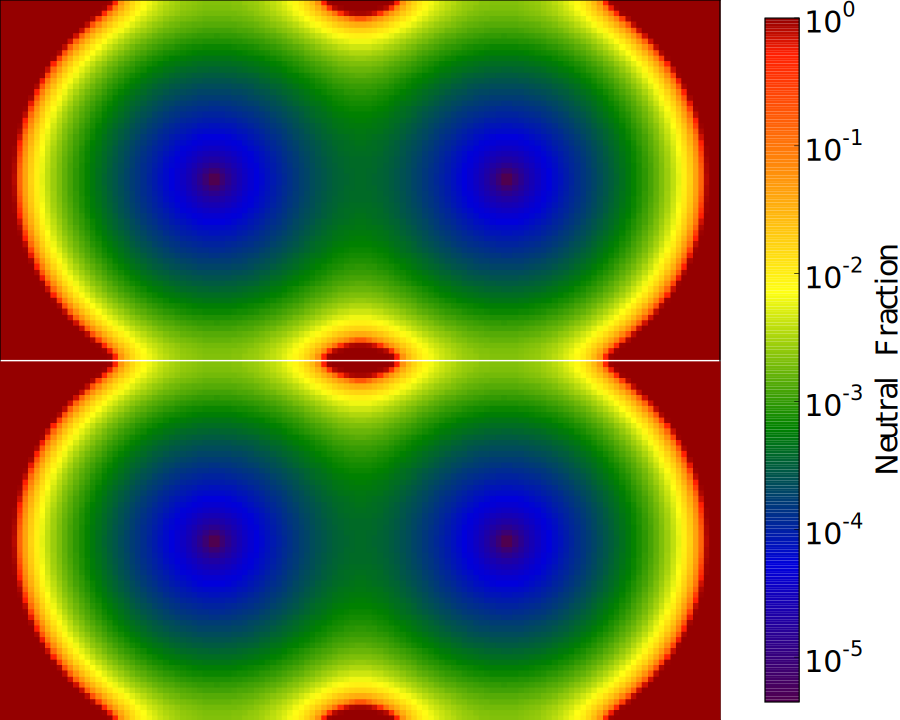
\includegraphics[scale=2.0, trim=0.0cm 0.0cm 0.0cm 0.0cm]{consolidated.png}
  }
  \caption{(Consolidated HII test) Slices of the neutral fraction at
    t=500 Myr through the sources from the ray-tracing solver.} 
  \label{fig:consolidated_RT}
\end{figure}

\begin{figure}[t]
  \centerline{
  \includegraphics[scale=0.35, trim=0.0cm 0.0cm 0.0cm 0.0cm]{consolidated_A.png}
  \includegraphics[scale=0.35, trim=0.0cm 0.0cm 0.0cm 0.0cm]{consolidated_B.png}
  }
  \centerline{
  \hfill
%  \includegraphics[scale=0.35, trim=0.0cm 0.0cm 0.0cm 0.0cm]{consolidated_C.png}
  \includegraphics[scale=0.35, trim=0.0cm 0.0cm 0.0cm 0.0cm]{consolidated_D.png}
  }
  \centerline{
  \includegraphics[scale=0.35, trim=1.0cm 0.0cm 1.0cm 0.0cm]{consolidated_E.png}
  \includegraphics[scale=0.35, trim=0.0cm 0.0cm 0.0cm 0.0cm]{consolidated_orig.png}
  }
  \caption{(Consolidated HII test) Slices of the neutral fraction at
    t=500 Myr through the sources from the FLD approaches: first row
    are approaches A and B; second is D, third are E and F.
    Approach C did not finish, so the results are not shown here;
    otherwise all approaches provide equally valid results.} 
  \label{fig:consolidated}
\end{figure}




\end{document}
